\noindent Đĩa Faraday là một máy phát điện đơn giản, có cấu tạo bao gồm một đĩa kim loại làm bằng sắt (một loại vật liệu dẫn điện) có bán kính trong là $r_1$, bán kính ngoài là $r_2$ và độ dày là $h$. \\
\begin{figure}[H]
  \centering
  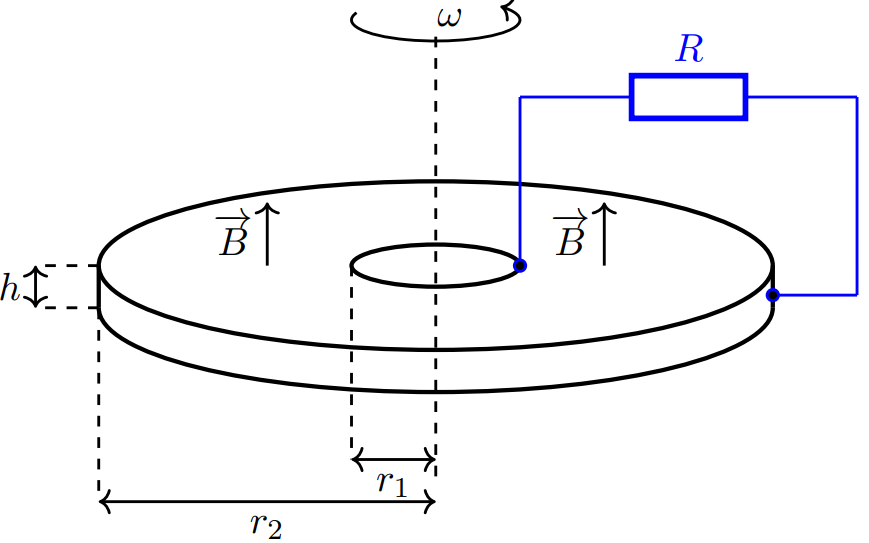
\includegraphics[width=0.5\textwidth]{Figures/Problems/Fig 1.1.png}
  \begin{center}
    \figurename{ 1}
  \end{center}
\end{figure}
\vspace{-0.5cm}
\noindent Đĩa được đặt trong một từ trường đều không đổi có cảm ứng từ $\vec{B}$ theo phương vuông góc với mặt phẳng của đĩa như được biểu diễn trong hình vẽ. Độ dẫn điện của sắt là $\sigma$.

\subsubsection*{Phần A: Mạch hở}
\noindent Trong phần này, người ta cho đĩa quay với tốc độ góc không đổi $\omega$ như Hình 1. Lúc này, đĩa chưa được nối với điện trở $R$ (không có đoạn mạch màu xanh dương).
\begin{enumerate}
  \item Xác định điện trường $\vec{E}$ bên trong đĩa và hiệu điện thế $V_0$ giữa mép trong và mép ngoài của đĩa. \textit{Gợi ý:} Trong một vật dẫn ở trạng thái cân bằng tĩnh điện, hợp lực tác dụng lên các điện tích tự do bằng không.
  \item Tìm điện trở $R_0$ của đĩa.
\end{enumerate}

\subsubsection*{Phần B: Phát điện}
\noindent Bây giờ, mép trong và mép ngoài của đĩa được nối với một điện trở $R$ như được minh họa bằng màu xanh dương trong hình vẽ. Các tiếp điểm không quay cùng với đĩa. Giả sử các tiếp điểm không có điện trở. Bỏ qua mọi ma sát.
\begin{enumerate}
  \item Xác định hiệu điện thế $V$ giữa mép trong và mép ngoài của đĩa. \textit{Gợi ý:} Lúc này, đĩa hoạt động như một nguồn điện không lý tưởng.
  \item Tính tổng công suất $P_0$ và công suất điện $P$ của nguồn.
  \item Tìm hiệu suất $\eta$ của máy phát.
  \item Tìm công suất điện cực đại $P_{\text{max}}$ và hiệu suất của nguồn khi hoạt động tại công suất đầu ra này.
\end{enumerate}

\subsubsection*{Phần C: Phanh tái sinh}
\noindent $N$ đĩa Faraday được dùng làm bánh xe và được kết nối cơ học với một đoàn tàu. Đoàn tàu có khối lượng $M = 400$ tấn và điện trở hiệu dụng $R$, mỗi bánh xe có khối lượng $m = 30$ kg. Phần duy nhất của tàu có chuyển động quay là các bánh xe. Sắt có độ dẫn điện $\sigma = 1{,}0 \cdot 10^7~\Omega^{-1} \cdot m^{-1}$, nhiệt dung riêng $c = 4{,}5 \cdot 10^2~J\,kg^{-1}\,K^{-1}$ và nhiệt độ nóng chảy $T = 1800~\text{K}$.
\begin{enumerate}
  \item Biểu diễn động năng của đoàn tàu dưới dạng $E = \frac{1}{2}I_{\text{eff}}\omega^2$ theo các đại lượng đã cho khi bánh xe quay với tốc độ góc $\omega$. Tìm $I_{\text{eff}}$. \textit{Gợi ý:} Moment quán tính của một vành tròn có khối lượng $M$, bán kính trong $R_1$ và bán kính ngoài $R_2$ đối với trục quay đi qua tâm và vuông góc với mặt phẳng vành là
        \begin{equation*}
          \frac{1}{2} M(R_2^2 + R_1^2)
        \end{equation*}
  \item Xác định động năng của đoàn tàu trong trường hợp $M \gg Nm$.
  \item Trong các ý còn lại của phần C, bạn có thể giả sử rằng $M \gg Nm$.
  \item Xác định tốc độ góc $\omega$ tại thời điểm $t$.
  \item Mất bao lâu để tốc độ của tàu giảm đi một nửa?
  \item Nếu tàu được hãm bằng cách nối tắt vành trong với vành ngoài của đĩa (lúc này $R = 0$), hãy ước lượng số lượng bánh xe tối thiểu để chúng không bị nóng chảy.
  \item Gia tốc khi hãm phanh có an toàn cho hành khách không? Lấy $B = 0{,}1\,$T, $r_1 = 10\,$cm, $r_2 = 50\,$cm và $h = 1{,}0\,$cm.
\end{enumerate}